\chapter{OFVA - Exercício 1} \label{Chap:AppendixB}


\begin{xltabular}{\textwidth}{|l|X|}
	\hline
	\endfirsthead
	
	\hline \multicolumn{2}{|c|}{continuação da página anterior} \\ \hline
	\endhead
	
	\hline \multicolumn{2}{|r|}{Continua na próxima página} \\ \hline
	\endfoot
	
	\hline
	\endlastfoot
	
	\multicolumn{2}{|c|}{\cellcolor[HTML]{C0C0C0}\textbf{ASPECTOS EDUCACIONAIS}} \\ \hline
	\textbf{NOME} & Quadro Trigonométrico - Quadrantes\\ \hline
	\textbf{DESCRIÇÃO GERAL} & Este objeto de aprendizagem trabalha com conceitos relacionados a Trigonometria, em especial, os valores dos quadrantes do círculo trigonométrico. \\ \hline
	\textbf{TÓPICOS} & Trigonometria, ângulos, círculo trigonométrico, quadrantes, graus, radianos\\ \hline
	\textbf{DESCRIÇÃO EDUCACIONAL} & No Player Virtual, o estudante deve escolher o item a ser estudado (início ou fim de um quadrante) e, então, deve manipular o ponteiro do Player Físico de modo a indicar a posição (ângulo) em que o quadrante começa ou termina (de acordo com o item escolhido). Para cada movimentação do ponteiro físico, o ponteiro virtual é movimentado e, após a confirmação da posição pelo estudante, é habilitada uma caixa de texto, onde deverão ser inseridos os valores do ângulo em graus e em radianos. Caso o aluno posicione o ponteiro físico em um local que não é um limite de quadrante, ou insira um valor incorreto, o Player Virtual deverá retornar uma informação que o ajude a corrigir os valores ou posições. Este objeto deve usar a Face A01 do OFVA Quadro Trigonométrico. \\ \hline
	\textbf{MODO} & ESTUDO \\ \hline
	\multicolumn{2}{|c|}{\cellcolor[HTML]{C0C0C0}\textbf{DISPOSITIVOS}} \\ \hline
	\textbf{ITENS} & 32 sensores de efeito hall; 1 imã de neodímio; ESP-WROOM-32; 1 Teclado membrana matricial; 1 Display LCD, Interface Wifi \\ \hline
	\multicolumn{2}{|c|}{\cellcolor[HTML]{C0C0C0}\textbf{RECURSOS}} \\ \hline
	\textbf{RECURSOS FÍSICOS} & .hex e .ino em Arduíno, Ponteiro físico, Face A01 (com círculo trigonométrico sem posições/valores de ângulos/quadrantes definidos)  \\ \hline
	\textbf{RECURSOS DIGITAIS} & Player Virtual \\ \hline		
	\multicolumn{2}{|c|}{\cellcolor[HTML]{C0C0C0}\textbf{SERVIÇOS}} \\ \hline
	\textbf{ITENS} & Iniciar atividade (botão), Leitura de hipertexto, Envio de resposta física (formato: websocket + json + botão físico), Envio de resposta digital (html tracking), Confirmação de resposta (visualização de respostas dadas), Feedback (modo estudo), Encerrar atividade (botão)  \\ \hline
	
\end{xltabular}

\begin{xltabular}{\textwidth}{|c|c|c|c|c|c|}
	\hline
	\endfirsthead
	
	\hline \multicolumn{6}{|c|}{continuação da página anterior} \\ \hline
	\endhead
	
	\hline \multicolumn{6}{|r|}{Continua na próxima página} \\ \hline
	\endfoot
	
	\hline
	\endlastfoot
	
	\multicolumn{6}{|c|}{\cellcolor[HTML]{C0C0C0}\textbf{ENTRADAS E SAÍDAS}} \\ \hline
	\multicolumn{6}{|c|}{\cellcolor[HTML]{DEDEDE}\textbf{CONJUNTO DE ENTRADAS}} \\ \hline
	\textbf{ID} & \textbf{FONTE} & \textbf{RÓTULO} & \textbf{TIPO DE DADO} & \textbf{BLOCOS} & \textbf{JavaScript} \\ \hline
	1 & Físico & EF1 & inteiro & \multicolumn{1}{|l|}{\begin{tabular}[c]{@{}l@{}} \\ 
\includegraphics[width=0.2\linewidth]{chapters/appendixC/entrada1.png}  \end{tabular} } & var EF1; \\ \hline
	2 & Virtual & EV1 & inteiro & \multicolumn{1}{|l|}{\begin{tabular}[c]{@{}l@{}} \\ 
\includegraphics[width=0.2\linewidth]{chapters/appendixC/entrada2.png}  \end{tabular} } & var EV1; \\ \hline
	3 & Virtual & EV2 & ponto flutuante & \multicolumn{1}{|l|}{\begin{tabular}[c]{@{}l@{}} \\ 
\includegraphics[width=0.2\linewidth]{chapters/appendixC/entrada3.png}  \end{tabular} } & var EV2; \\ \hline
	\multicolumn{6}{|c|}{\cellcolor[HTML]{DEDEDE}\textbf{CONJUNTO DE SAÍDAS}} \\ \hline
	\textbf{ID} & \textbf{FONTE} & \textbf{RÓTULO} & \textbf{TIPO DE DADO} &  \multicolumn{2}{|c|}{\textbf{CONTEÚDO}} \\ \hline
	1 & Virtual & SV1 & String & \multicolumn{2}{|l|}{Mova o ponteiro no sentido horário} \\ \hline
	2 & Virtual & SV2 & String & \multicolumn{2}{|l|}{Mova o ponteiro no sentido anti-horário} \\ \hline
	3 & Virtual & SV3 & String & \multicolumn{2}{|l|}{Posição está correta!} \\ \hline
	4 & Virtual & SV4 & String & \multicolumn{2}{|l|}{\begin{tabular}[c]{@{}l@{}} Ao menos um dos valores informados \\deveria ser menor \end{tabular}} \\ \hline
	5 & Virtual & SV5 & String & \multicolumn{2}{|l|}{\begin{tabular}[c]{@{}l@{}} Ao menos um dos valores informados \\deveria ser maior \end{tabular}} \\ \hline
	6 & Virtual & SV6 & String & \multicolumn{2}{|l|}{Todos os valores estão corretos!} \\ \hline	
	\multicolumn{6}{|c|}{\textbf{BLOCOS}} \\ \hline
	\multicolumn{6}{|c|}{\begin{tabular}[c]{@{}l@{}} \\ 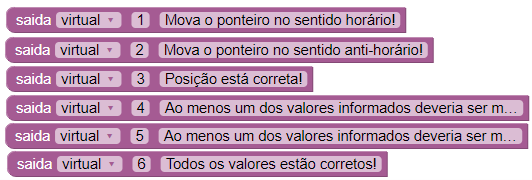
\includegraphics[width=0.8\linewidth]{chapters/appendixC/saidas.png}  \end{tabular}} \\ \hline
	\multicolumn{6}{|c|}{\textbf{JavaScript gerado}} \\ \hline
	\multicolumn{6}{|l|}{\begin{tabular}[c]{@{}l@{}} var SV1 = "Mova o ponteiro no sentido horário!";\\ 			var SV2 = "Mova o ponteiro no sentido anti-horário!";\\ 			var SV3 = "Posição está correta!";\\ 			var SV4 = "Ao menos um dos valores informados deveria ser menor";\\			var SV5 = "Ao menos um dos valores informados deveria ser maior";\\			var SV6 = "Todos os valores estão corretos!"; \end{tabular}} \\ \hline
	
\end{xltabular}

\begin{xltabular}{\textwidth}{|c|X|}
	\hline
	\endfirsthead
	
	\hline \multicolumn{2}{|c|}{continuação da página anterior} \\ \hline
	\endhead
	
	\hline \multicolumn{2}{|r|}{Continua na próxima página} \\ \hline
	\endfoot
	
	\hline
	\endlastfoot
	
	\multicolumn{2}{|c|}{\cellcolor[HTML]{C0C0C0}\textbf{CASOS DE TESTE}} \\ \hline

%CASO 1
\multicolumn{2}{|c|}{\cellcolor[HTML]{DEDEDE}\textbf{CASO DE TESTE 1}} \\ \hline
\multicolumn{1}{|l|}{\textbf{Rótulo:}} & INÍCIO \\ \hline
\multicolumn{1}{|l|}{\textbf{Situação-problema (Enunciado):}} & Indique o início do primeiro quadrante e informe seu valor em grau e radiano.\\ \hline
\multicolumn{2}{|c|}{\cellcolor[HTML]{DEDEDE}\textbf{REGRA 1}} \\ \hline
\textbf{Blocos} & \multicolumn{1}{c|}{\textbf{JavaScript gerado}} \\ \hline
\multicolumn{1}{|l|}{\begin{tabular}[c]{@{}l@{}} \\ 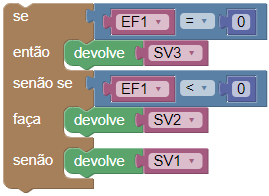
\includegraphics[width=0.4\linewidth]{chapters/appendixB/c1r1.png}  \end{tabular}
} & \begin{tabular}[c]{@{}l@{}} if((EF1 == 0))\{   return SV3; \}\\ else if ((EF1 < 0))\{   return SV2; \}\\ else \{   return SV1; \} \end{tabular} \\ \hline
\multicolumn{2}{|c|}{\cellcolor[HTML]{DEDEDE}\textbf{REGRA 2}} \\ \hline
\textbf{Blocos} & \multicolumn{1}{c|}{\textbf{JavaScript gerado}} \\ \hline
\multicolumn{1}{|l|}{\begin{tabular}[c]{@{}l@{}} \\ 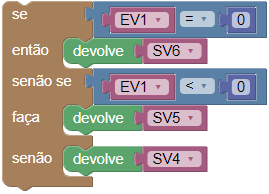
\includegraphics[width=0.4\linewidth]{chapters/appendixB/c1r2.png}  \end{tabular}
} &  \begin{tabular}[c]{@{}l@{}}if((EV1 == 0))\{   return SV6; \}\\ else if ((EV1 < 0))\{   return SV5; \}\\ else \{   return SV4; \} \end{tabular}  \\ \hline
\multicolumn{2}{|c|}{\cellcolor[HTML]{DEDEDE}\textbf{REGRA 3}} \\ \hline
\textbf{Blocos} & \multicolumn{1}{c|}{\textbf{JavaScript gerado}} \\ \hline
\multicolumn{1}{|l|}{\begin{tabular}[c]{@{}l@{}} \\ 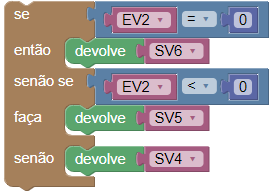
\includegraphics[width=0.4\linewidth]{chapters/appendixB/c1r3.png}  \end{tabular}
} & \begin{tabular}[c]{@{}l@{}}if((EV2 == 0))\{   return SV6; \}\\ else if ((EV2 < 0))\{   return SV5; \}\\ else \{   return SV4; \} \end{tabular}  \\ \hline


	
%CASO 2
	\multicolumn{2}{|c|}{\cellcolor[HTML]{DEDEDE}\textbf{CASO DE TESTE 2}} \\ \hline
	\multicolumn{1}{|l|}{\textbf{Rótulo:}} & FIM \\ \hline
	\multicolumn{1}{|l|}{\textbf{Situação-problema (Enunciado):}} & Indique o fim do primeiro quadrante e informe seu valor em grau e radiano.\\ \hline
	\multicolumn{2}{|c|}{\cellcolor[HTML]{DEDEDE}\textbf{REGRA 1}} \\ \hline
	\textbf{Blocos} & \multicolumn{1}{c|}{\textbf{JavaScript gerado}} \\ \hline
	\multicolumn{1}{|l|}{\begin{tabular}[c]{@{}l@{}} \\ 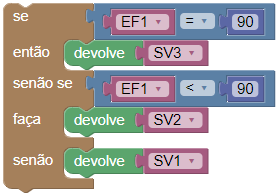
\includegraphics[width=0.5\linewidth]{chapters/appendixB/c2r1.png}  \end{tabular}
	} & \begin{tabular}[c]{@{}l@{}} if((EF1 == 90))\{   return SV3; \}\\ else if ((EF1 < 90))\{   return SV2; \}\\ else \{   return SV1; \} \end{tabular} \\ \hline
	\multicolumn{2}{|c|}{\cellcolor[HTML]{DEDEDE}\textbf{REGRA 2}} \\ \hline
	\textbf{Blocos} & \multicolumn{1}{c|}{\textbf{JavaScript gerado}} \\ \hline
	\multicolumn{1}{|l|}{\begin{tabular}[c]{@{}l@{}} \\ 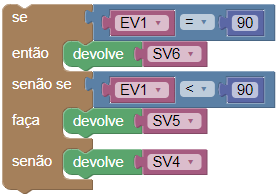
\includegraphics[width=0.4\linewidth]{chapters/appendixB/c2r2.png}  \end{tabular}
	} &  \begin{tabular}[c]{@{}l@{}}if((EV1 == 90))\{   return SV6; \}\\ else if ((EV1 < 90))\{   return SV5; \}\\ else \{   return SV4; \} \end{tabular}  \\ \hline
	\multicolumn{2}{|c|}{\cellcolor[HTML]{DEDEDE}\textbf{REGRA 3}} \\ \hline
	\textbf{Blocos} & \multicolumn{1}{c|}{\textbf{JavaScript gerado}} \\ \hline
	\multicolumn{1}{|l|}{\begin{tabular}[c]{@{}l@{}} \\ 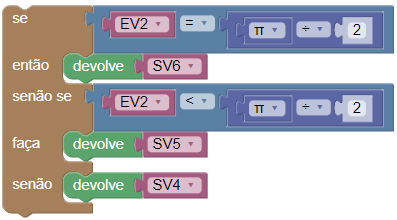
\includegraphics[width=0.4\linewidth]{chapters/appendixB/c2r3.png}  \end{tabular}
	} & \begin{tabular}[c]{@{}l@{}}if((EV2 == Math.PI / 2))\{   return SV6; \}\\ else if ((EV2 < Math.PI / 2))\{   return SV5; \}\\ else \{   return SV4; \} \end{tabular}  \\ \hline

%CASO 3
\multicolumn{2}{|c|}{\cellcolor[HTML]{DEDEDE}\textbf{CASO DE TESTE 3}} \\ \hline
\multicolumn{1}{|l|}{\textbf{Rótulo:}} & INÍCIO \\ \hline
\multicolumn{1}{|l|}{\textbf{Situação-problema (Enunciado):}} & Indique o início do segundo quadrante e informe seu valor em grau e radiano.\\ \hline
\multicolumn{2}{|c|}{\cellcolor[HTML]{DEDEDE}\textbf{REGRA 1}} \\ \hline
\textbf{Blocos} & \multicolumn{1}{c|}{\textbf{JavaScript gerado}} \\ \hline
\multicolumn{1}{|l|}{\begin{tabular}[c]{@{}l@{}} \\ 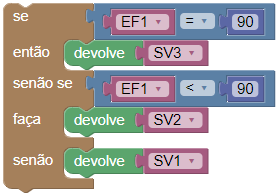
\includegraphics[width=0.4\linewidth]{chapters/appendixB/c2r1.png}  \end{tabular}
} & \begin{tabular}[c]{@{}l@{}} if((EF1 == 90))\{   return SV3; \}\\ else if ((EF1 < 90))\{   return SV2; \}\\ else \{   return SV1; \} \end{tabular} \\ \hline
\multicolumn{2}{|c|}{\cellcolor[HTML]{DEDEDE}\textbf{REGRA 2}} \\ \hline
\textbf{Blocos} & \multicolumn{1}{c|}{\textbf{JavaScript gerado}} \\ \hline
\multicolumn{1}{|l|}{\begin{tabular}[c]{@{}l@{}} \\ 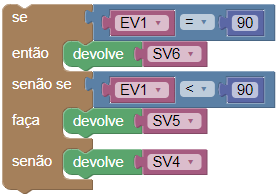
\includegraphics[width=0.4\linewidth]{chapters/appendixB/c2r2.png}  \end{tabular}
} &  \begin{tabular}[c]{@{}l@{}}if((EV1 == 90))\{   return SV6; \}\\ else if ((EV1 < 90))\{   return SV5; \}\\ else \{   return SV4; \} \end{tabular}  \\ \hline
\multicolumn{2}{|c|}{\cellcolor[HTML]{DEDEDE}\textbf{REGRA 3}} \\ \hline
\textbf{Blocos} & \multicolumn{1}{c|}{\textbf{JavaScript gerado}} \\ \hline
\multicolumn{1}{|l|}{\begin{tabular}[c]{@{}l@{}} \\ 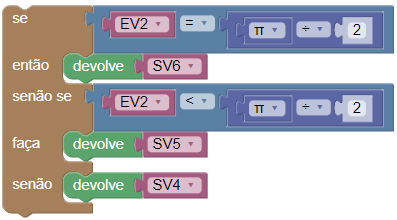
\includegraphics[width=0.4\linewidth]{chapters/appendixB/c2r3.png}  \end{tabular}
} & \begin{tabular}[c]{@{}l@{}}if((EV2 == Math.PI / 2))\{   return SV6; \}\\ else if ((EV2 < Math.PI / 2))\{   return SV5; \}\\ else \{   return SV4; \} \end{tabular}  \\ \hline


%CASO 4
\multicolumn{2}{|c|}{\cellcolor[HTML]{DEDEDE}\textbf{CASO DE TESTE 4}} \\ \hline
\multicolumn{1}{|l|}{\textbf{Rótulo:}} & FIM \\ \hline
\multicolumn{1}{|l|}{\textbf{Situação-problema (Enunciado):}} & Indique o fim do segundo quadrante e informe seu valor em grau e radiano.\\ \hline
\multicolumn{2}{|c|}{\cellcolor[HTML]{DEDEDE}\textbf{REGRA 1}} \\ \hline
\textbf{Blocos} & \multicolumn{1}{c|}{\textbf{JavaScript gerado}} \\ \hline
\multicolumn{1}{|l|}{\begin{tabular}[c]{@{}l@{}} \\ 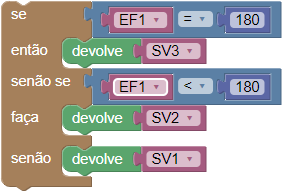
\includegraphics[width=0.4\linewidth]{chapters/appendixB/c4r1.png}  \end{tabular}
} & \begin{tabular}[c]{@{}l@{}} if((EF1 == 180))\{   return SV3; \}\\ else if ((EF1 < 180))\{   return SV2; \}\\ else \{   return SV1; \} \end{tabular} \\ \hline
\multicolumn{2}{|c|}{\cellcolor[HTML]{DEDEDE}\textbf{REGRA 2}} \\ \hline
\textbf{Blocos} & \multicolumn{1}{c|}{\textbf{JavaScript gerado}} \\ \hline
\multicolumn{1}{|l|}{\begin{tabular}[c]{@{}l@{}} \\ 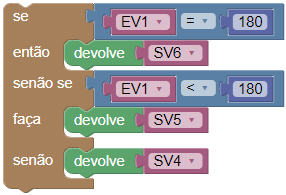
\includegraphics[width=0.4\linewidth]{chapters/appendixB/c4r2.png}  \end{tabular}
} &  \begin{tabular}[c]{@{}l@{}}if((EV1 == 180))\{   return SV6; \}\\ else if ((EV1 < 180))\{   return SV5; \}\\ else \{   return SV4; \} \end{tabular}  \\ \hline
\multicolumn{2}{|c|}{\cellcolor[HTML]{DEDEDE}\textbf{REGRA 3}} \\ \hline
\textbf{Blocos} & \multicolumn{1}{c|}{\textbf{JavaScript gerado}} \\ \hline
\multicolumn{1}{|l|}{\begin{tabular}[c]{@{}l@{}} \\ 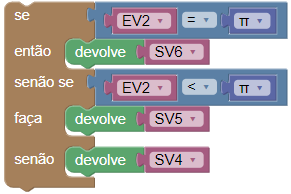
\includegraphics[width=0.4\linewidth]{chapters/appendixB/c4r3.png}  \end{tabular}
} & \begin{tabular}[c]{@{}l@{}}if((EV2 == Math.PI))\{   return SV6; \}\\ else if ((EV2 < Math.PI))\{   return SV5; \}\\ else \{   return SV4; \} \end{tabular}  \\ \hline
	
%CASO 5
\multicolumn{2}{|c|}{\cellcolor[HTML]{DEDEDE}\textbf{CASO DE TESTE 5}} \\ \hline
\multicolumn{1}{|l|}{\textbf{Rótulo:}} & INÍCIO \\ \hline
\multicolumn{1}{|l|}{\textbf{Situação-problema (Enunciado):}} & Indique o início do terceiro quadrante e informe seu valor em grau e radiano.\\ \hline
\multicolumn{2}{|c|}{\cellcolor[HTML]{DEDEDE}\textbf{REGRA 1}} \\ \hline
\textbf{Blocos} & \multicolumn{1}{c|}{\textbf{JavaScript gerado}} \\ \hline
\multicolumn{1}{|l|}{\begin{tabular}[c]{@{}l@{}} \\ 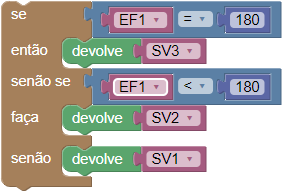
\includegraphics[width=0.4\linewidth]{chapters/appendixB/c4r1.png}  \end{tabular}
} & \begin{tabular}[c]{@{}l@{}} if((EF1 == 180))\{   return SV3; \}\\ else if ((EF1 < 180))\{   return SV2; \}\\ else \{   return SV1; \} \end{tabular} \\ \hline
\multicolumn{2}{|c|}{\cellcolor[HTML]{DEDEDE}\textbf{REGRA 2}} \\ \hline
\textbf{Blocos} & \multicolumn{1}{c|}{\textbf{JavaScript gerado}} \\ \hline
\multicolumn{1}{|l|}{\begin{tabular}[c]{@{}l@{}} \\ 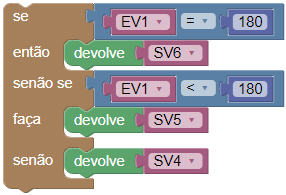
\includegraphics[width=0.4\linewidth]{chapters/appendixB/c4r2.png}  \end{tabular}
} &  \begin{tabular}[c]{@{}l@{}}if((EV1 == 180))\{   return SV6; \}\\ else if ((EV1 < 180))\{   return SV5; \}\\ else \{   return SV4; \} \end{tabular}  \\ \hline
\multicolumn{2}{|c|}{\cellcolor[HTML]{DEDEDE}\textbf{REGRA 3}} \\ \hline
\textbf{Blocos} & \multicolumn{1}{c|}{\textbf{JavaScript gerado}} \\ \hline
\multicolumn{1}{|l|}{\begin{tabular}[c]{@{}l@{}} \\ 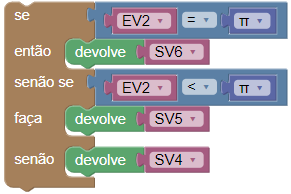
\includegraphics[width=0.4\linewidth]{chapters/appendixB/c4r3.png}  \end{tabular}
} & \begin{tabular}[c]{@{}l@{}}if((EV2 == Math.PI))\{   return SV6; \}\\ else if ((EV2 < Math.PI))\{   return SV5; \}\\ else \{   return SV4; \} \end{tabular}  \\ \hline	

%CASO 6
\multicolumn{2}{|c|}{\cellcolor[HTML]{DEDEDE}\textbf{CASO DE TESTE 6}} \\ \hline
\multicolumn{1}{|l|}{\textbf{Rótulo:}} & FIM \\ \hline
\multicolumn{1}{|l|}{\textbf{Situação-problema (Enunciado):}} & Indique o fim do terceiro quadrante e informe seu valor em grau e radiano.\\ \hline
\multicolumn{2}{|c|}{\cellcolor[HTML]{DEDEDE}\textbf{REGRA 1}} \\ \hline
\textbf{Blocos} & \multicolumn{1}{c|}{\textbf{JavaScript gerado}} \\ \hline
\multicolumn{1}{|l|}{\begin{tabular}[c]{@{}l@{}} \\ 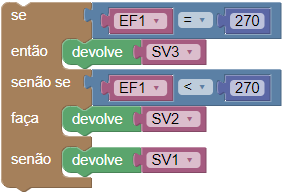
\includegraphics[width=0.4\linewidth]{chapters/appendixB/c6r1.png}  \end{tabular}
} & \begin{tabular}[c]{@{}l@{}} if((EF1 == 270))\{   return SV3; \}\\ else if ((EF1 < 270))\{   return SV2; \}\\ else \{   return SV1; \} \end{tabular} \\ \hline
\multicolumn{2}{|c|}{\cellcolor[HTML]{DEDEDE}\textbf{REGRA 2}} \\ \hline
\textbf{Blocos} & \multicolumn{1}{c|}{\textbf{JavaScript gerado}} \\ \hline
\multicolumn{1}{|l|}{\begin{tabular}[c]{@{}l@{}} \\ 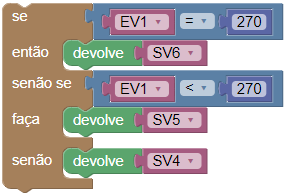
\includegraphics[width=0.4\linewidth]{chapters/appendixB/c6r2.png}  \end{tabular}
} &  \begin{tabular}[c]{@{}l@{}}if((EV1 == 270))\{   return SV6; \}\\ else if ((EV1 < 270))\{   return SV5; \}\\ else \{   return SV4; \} \end{tabular}  \\ \hline
\multicolumn{2}{|c|}{\cellcolor[HTML]{DEDEDE}\textbf{REGRA 3}} \\ \hline
\textbf{Blocos} & \multicolumn{1}{c|}{\textbf{JavaScript gerado}} \\ \hline
\multicolumn{1}{|l|}{\begin{tabular}[c]{@{}l@{}} \\ 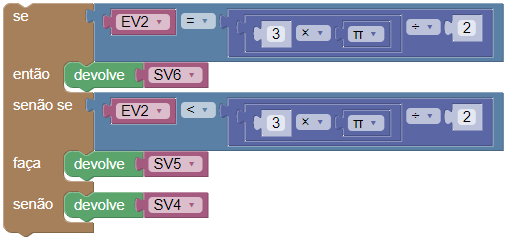
\includegraphics[width=0.4\linewidth]{chapters/appendixB/c6r3.png}  \end{tabular}
} & if((EV2 == (3 * Math.PI) / 2))\{   return SV6; \} else if ((EV2 < (3 * Math.PI) / 2))\{   return SV5; \} else \{   return SV4; \} \\ \hline	

%CASO 7
\multicolumn{2}{|c|}{\cellcolor[HTML]{DEDEDE}\textbf{CASO DE TESTE 7}} \\ \hline
\multicolumn{1}{|l|}{\textbf{Rótulo:}} & INÍCIO \\ \hline
\multicolumn{1}{|l|}{\textbf{Situação-problema (Enunciado):}} & Indique o início do quarto quadrante e informe seu valor em grau e radiano.\\ \hline
\multicolumn{2}{|c|}{\cellcolor[HTML]{DEDEDE}\textbf{REGRA 1}} \\ \hline
\textbf{Blocos} & \multicolumn{1}{c|}{\textbf{JavaScript gerado}} \\ \hline
\multicolumn{1}{|l|}{\begin{tabular}[c]{@{}l@{}} \\ 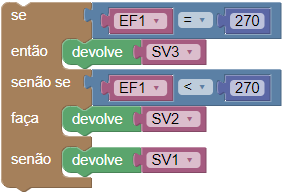
\includegraphics[width=0.4\linewidth]{chapters/appendixB/c6r1.png}  \end{tabular}
} & \begin{tabular}[c]{@{}l@{}} if((EF1 == 270))\{   return SV3; \}\\ else if ((EF1 < 270))\{   return SV2; \}\\ else \{   return SV1; \} \end{tabular} \\ \hline
\multicolumn{2}{|c|}{\cellcolor[HTML]{DEDEDE}\textbf{REGRA 2}} \\ \hline
\textbf{Blocos} & \multicolumn{1}{c|}{\textbf{JavaScript gerado}} \\ \hline
\multicolumn{1}{|l|}{\begin{tabular}[c]{@{}l@{}} \\ 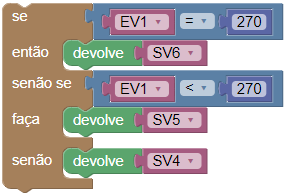
\includegraphics[width=0.4\linewidth]{chapters/appendixB/c6r2.png}  \end{tabular}
} &  \begin{tabular}[c]{@{}l@{}}if((EV1 == 270))\{   return SV6; \}\\ else if ((EV1 < 270))\{   return SV5; \}\\ else \{   return SV4; \} \end{tabular}  \\ \hline
\multicolumn{2}{|c|}{\cellcolor[HTML]{DEDEDE}\textbf{REGRA 3}} \\ \hline
\textbf{Blocos} & \multicolumn{1}{c|}{\textbf{JavaScript gerado}} \\ \hline
\multicolumn{1}{|l|}{\begin{tabular}[c]{@{}l@{}} \\ 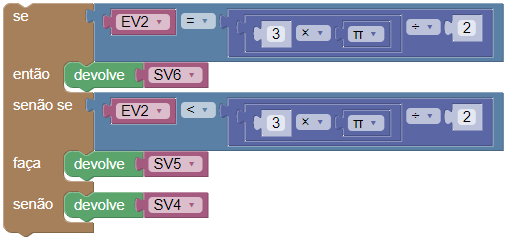
\includegraphics[width=0.4\linewidth]{chapters/appendixB/c6r3.png}  \end{tabular}
} & if((EV2 == (3 * Math.PI) / 2))\{   return SV6; \} else if ((EV2 < (3 * Math.PI) / 2))\{   return SV5; \} else \{   return SV4; \} \\ \hline	

%CASO 8
\multicolumn{2}{|c|}{\cellcolor[HTML]{DEDEDE}\textbf{CASO DE TESTE 8}} \\ \hline
\multicolumn{1}{|l|}{\textbf{Rótulo:}} & FIM \\ \hline
\multicolumn{1}{|l|}{\textbf{Situação-problema (Enunciado):}} & Indique o fim do quarto quadrante e informe seu valor em grau e radiano.\\ \hline
\multicolumn{2}{|c|}{\cellcolor[HTML]{DEDEDE}\textbf{REGRA 1}} \\ \hline
\textbf{Blocos} & \multicolumn{1}{c|}{\textbf{JavaScript gerado}} \\ \hline
\multicolumn{1}{|l|}{\begin{tabular}[c]{@{}l@{}} \\ 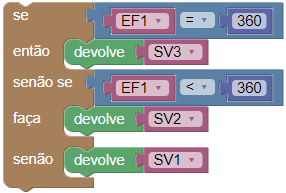
\includegraphics[width=0.4\linewidth]{chapters/appendixB/c8r1.png}  \end{tabular}
} & \begin{tabular}[c]{@{}l@{}} if((EF1 == 360))\{   return SV3; \}\\ else if ((EF1 < 360))\{   return SV2; \}\\ else \{   return SV1; \} \end{tabular} \\ \hline
\multicolumn{2}{|c|}{\cellcolor[HTML]{DEDEDE}\textbf{REGRA 2}} \\ \hline
\textbf{Blocos} & \multicolumn{1}{c|}{\textbf{JavaScript gerado}} \\ \hline
\multicolumn{1}{|l|}{\begin{tabular}[c]{@{}l@{}} \\ 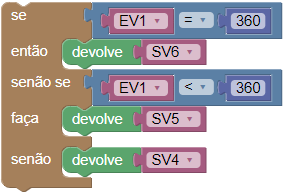
\includegraphics[width=0.4\linewidth]{chapters/appendixB/c8r2.png}  \end{tabular}
} &  \begin{tabular}[c]{@{}l@{}}if((EV1 == 360))\{   return SV6; \}\\ else if ((EV1 < 360))\{   return SV5; \}\\ else \{   return SV4; \} \end{tabular}  \\ \hline
\multicolumn{2}{|c|}{\cellcolor[HTML]{DEDEDE}\textbf{REGRA 3}} \\ \hline
\textbf{Blocos} & \multicolumn{1}{c|}{\textbf{JavaScript gerado}} \\ \hline
\multicolumn{1}{|l|}{\begin{tabular}[c]{@{}l@{}} \\ 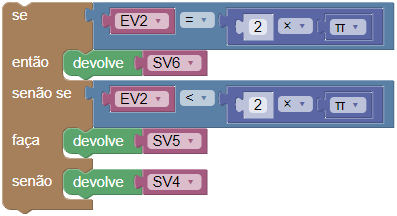
\includegraphics[width=0.4\linewidth]{chapters/appendixB/c8r3.png}  \end{tabular}
} & if((EV2 == (2 * Math.PI)))\{   return SV6; \} else if ((EV2 < (2 * Math.PI)))\{   return SV5; \} else \{   return SV4; \} \\ \hline	
	
\end{xltabular}

\begin{xltabular}{\textwidth}{|l|c|}
	\hline
	\endfirsthead
	
	\hline \multicolumn{2}{|c|}{continuação da página anterior} \\ \hline
	\endhead
	
	\hline \multicolumn{2}{|r|}{Continua na próxima página} \\ \hline
	\endfoot
	
	\hline
	\endlastfoot
	
	\cellcolor[HTML]{C0C0C0}\textbf{AGRUPAR CASOS DE TESTE?} & SIM \\ \hline
	\cellcolor[HTML]{DEDEDE}\textbf{ID GRUPO} & \cellcolor[HTML]{DEDEDE}1\\ \hline
	\textbf{RÓTULO} & QUADRANTE 1 \\ \hline
	\textbf{AGRUPAMENTO} & \{1,2\}\\ \hline
	\cellcolor[HTML]{DEDEDE}\textbf{ID GRUPO} & \cellcolor[HTML]{DEDEDE}2\\ \hline
	\textbf{RÓTULO} & QUADRANTE 2 \\ \hline
	\textbf{AGRUPAMENTO} & \{3,4\}\\ \hline
	\cellcolor[HTML]{DEDEDE}\textbf{ID GRUPO} & \cellcolor[HTML]{DEDEDE}3\\ \hline
	\textbf{RÓTULO} & QUADRANTE 3 \\ \hline
	\textbf{AGRUPAMENTO} & \{5,6\}\\ \hline
	\cellcolor[HTML]{DEDEDE}\textbf{ID GRUPO} & \cellcolor[HTML]{DEDEDE}4\\ \hline
	\textbf{RÓTULO} & QUADRANTE 4 \\ \hline
	\textbf{AGRUPAMENTO} & \{7,8\}\\ \hline	
\end{xltabular}